\section{Transform Coding and JPEG}


\begin{questionbox}{Domanda 18}
Why the geometric mean of the variances of a random vector is key information to evaluate the rate-distortion performance of a quantizer?
\end{questionbox}


\begin{itemize}
  \item High-resolution transform coding with optimal bit allocation:

\end{itemize}
$$
D^\star = c_{GM}\sigma_{GM}^2 2^{-2\bar{R}}
$$

\begin{itemize}
  \item Orthogonal transforms preserve total energy $\rightarrow$ preserve arithmetic mean:

\end{itemize}
$$
\sigma_{AM,Y}^2 = \sigma_{AM,X}^2
$$

\begin{itemize}
  \item Transform can change variance distribution.
  \item \textbf{Good transform} $\rightarrow$ few high-energy coefficients, many low-energy coefficients $\rightarrow$ lower $\sigma_{GM}^2$.

\end{itemize}
$$
\sigma_{GM}^2 \le \sigma_{AM}^2
$$

\begin{itemize}
  \item \textbf{Lower geometric mean} $\rightarrow$ lower distortion at same rate.

\end{itemize}
$$
G_T = \frac{D_{\text{PCM}}}{D_Y}
=\frac{\sigma_{AM,Y}^2}{\sigma_{GM,Y}^2}
$$

$$
G_{T,dB}=10\log_{10}G_T
$$

\begin{questionbox}{Domanda 19}
Write the resource allocation problem for transform coding. Derive the Huang-Schulteiss formula.
\end{questionbox}


\begin{itemize}
  \item \textbf{High-resolution distortion}:

\end{itemize}
$$
D = \frac{1}{M}\sum_{k=0}^{M-1} c_k\sigma_k^2 2^{-2R_k}
$$

\begin{itemize}
  \item \textbf{Rate constraint}:

\end{itemize}
$$
\sum_{k=0}^{M-1} R_k \le R_{\text{tot}}
$$

\begin{itemize}
  \item \textbf{Lagrangian}:

\end{itemize}
$$
J(\vec{R},\lambda)=
\frac{1}{M}\sum_{k=0}^{M-1} c_k\sigma_k^2 2^{-2R_k}
+\lambda\left(\sum_{k=0}^{M-1}R_k-R_{\text{tot}}\right)
$$

\begin{itemize}
  \item Set $\frac{\partial J}{\partial R_k}=0$ $\rightarrow$ Huang-Schultheiss:

\end{itemize}
$$
R_k^\star = \frac{R_{\text{tot}}}{M}
+\frac{1}{2}\log_2\left(
\frac{c_k\sigma_k^2}{c_{GM}\sigma_{GM}^2}
\right)
$$

$$
c_{GM}=\sqrt[M]{\prod_{k=0}^{M-1} c_k},
\quad
\sigma_{GM}^2=\sqrt[M]{\prod_{k=0}^{M-1}\sigma_k^2}
$$

\begin{itemize}
  \item \textbf{Above geometric mean} $\rightarrow$ more bits.
  \item \textbf{Below geometric mean} $\rightarrow$ fewer bits.

\end{itemize}
\begin{questionbox}{Domanda 20}
Explain why the KLT is the optimal linear transform for decorrelation and why the DCT is used in practice instead.
\end{questionbox}


\begin{itemize}
  \item \textbf{KLT} $\rightarrow$ eigenvectors of signal covariance matrix.
  \item \textbf{In KLT basis} $\rightarrow$ coefficients decorrelated; optimal energy compaction among linear orthogonal transforms for given statistics.

\end{itemize}
$$
T_{KLT} = [u_1\ u_2\ \cdots\ u_M]^T
$$

\begin{itemize}
  \item \textbf{Problem} $\rightarrow$ KLT depends on actual image/block statistics; encoder must estimate covariance, compute transform, signal it.
  \item \textbf{DCT} used because fixed, separable, fast, no side information, good KLT approximation for locally correlated image blocks.

\end{itemize}
\begin{questionbox}{Domanda 21}
Describe the principles of the JPEG standard.
\end{questionbox}


\begin{itemize}
  \item \textbf{JPEG} $\rightarrow$ lossy still-image codec based on block DCT, quantization, entropy coding.
  \item Standard mainly defines decodable bitstream and decoder behavior; encoder choices flexible.

\end{itemize}
\begin{figure}[H]
\centering
\begin{tikzpicture}[
    block/.style={draw, rectangle, minimum width=2.2cm, minimum height=0.8cm, align=center, rounded corners=3pt, fill=blue!10, draw=blue!50!black, font=\small},
    arrow/.style={-latex, thick, draw=blue!50!black}
]
    \node [block] (rgb) {RGB};
    \node [block, right=0.8cm of rgb] (ycbcr) {YCbCr};
    \node [block, right=0.8cm of ycbcr] (chroma) {Chroma\\subsampling};
    \node [block, right=0.8cm of chroma] (blocks) {8x8 blocks};
    \node [block, right=0.8cm of blocks] (shift) {Level shift\\by 128};
    
    \node [block, below=1.2cm of shift] (dct) {DCT};
    \node [block, left=0.8cm of dct] (quant) {Quantization};
    \node [block, left=0.8cm of quant] (zigzag) {Zig-zag scan};
    \node [block, left=0.8cm of zigzag] (rle) {RLE/Huffman};
    \node [block, left=0.8cm of rle] (stream) {JPEG bitstream};
    
    \draw [arrow] (rgb) -- (ycbcr);
    \draw [arrow] (ycbcr) -- (chroma);
    \draw [arrow] (chroma) -- (blocks);
    \draw [arrow] (blocks) -- (shift);
    
    \draw [arrow] (shift.south) -- ++(0,-0.4) -| (dct.north);
    
    \draw [arrow] (dct) -- (quant);
    \draw [arrow] (quant) -- (zigzag);
    \draw [arrow] (zigzag) -- (rle);
    \draw [arrow] (rle) -- (stream);
\end{tikzpicture}
\caption{JPEG Coding Pipeline}
\label{fig:jpeg_pipeline}
\end{figure}

\begin{itemize}
  \item \textbf{Quantization}:

\end{itemize}
$$
\tilde{C}_{ij}=\text{round}\left(\frac{C_{ij}}{q_{ij}}\right)
$$

\begin{itemize}
  \item \textbf{Quantization table} $\rightarrow$ smaller steps for important low frequencies, larger steps for high frequencies.
  \item \textbf{Quality factor}:

\end{itemize}
$$
S_F =
\begin{cases}
\frac{5000}{Q} & 1 \le Q \le 50\\
200-2Q & 50 < Q \le 99\\
1 & Q=100
\end{cases}
$$

$$
q \leftarrow \frac{S_F}{100}q^\star
$$

\begin{itemize}
  \item \textbf{Metadata}:
  \begin{itemize}
    \item \textbf{JFIF} $\rightarrow$ density, resolution, thumbnails;
    \item \textbf{EXIF} $\rightarrow$ date/time, GPS, camera settings.

  \end{itemize}
\end{itemize}
\begin{questionbox}{Domanda 22}
(TC\&JPEG) Draw the scheme and describe the functional blocks of a JPEG encoder.
\end{questionbox}


\begin{figure}[H]
\centering
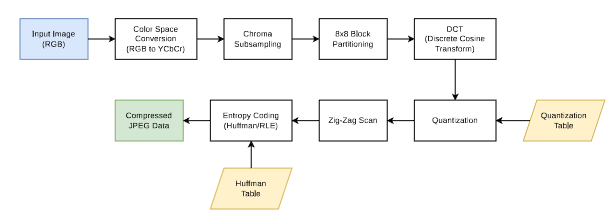
\includegraphics[width=0.75\textwidth]{images/JPEG_encoder.png}
\caption{JPEG encoder.png}
\end{figure}

\begin{itemize}
  \item \textbf{DCT} $\rightarrow$ energy compaction.
  \item \textbf{Quantization} $\rightarrow$ lossy coefficient reduction.
  \item \textbf{Zig-zag scan} $\rightarrow$ groups zeros.
  \item \textbf{Entropy coding} $\rightarrow$ lossless compression.

\end{itemize}
\begin{questionbox}{Domanda 23}
(TC\&JPEG) Describe the problem of “frequency leakage” in the Discrete Fourier Transform (DFT) when applied to signal compression and how the Discrete Cosine Transform (DCT) addresses it.
\end{questionbox}


\begin{itemize}
  \item DFT assumes finite signal is periodic.
  \item \textbf{Boundary mismatch} $\rightarrow$ artificial discontinuities $\rightarrow$ energy spread to high frequencies = \textbf{frequency leakage}.
  \item \textbf{DCT uses symmetric extension} $\rightarrow$ smoother periodic continuation $\rightarrow$ better energy compaction for images.

\end{itemize}
\begin{questionbox}{Domanda 24}
(TC\&JPEG) Explain the entropy coding process for AC coefficients in the JPEG standard and the significance of the “End of Block” (EOB) symbol.
\end{questionbox}


\begin{itemize}
  \item \textbf{After zig-zag scan, AC coefficients} $\rightarrow$ pairs:

\end{itemize}
$$
(r,k)
$$

\begin{itemize}
  \item $r$ $\rightarrow$ run of preceding zeros.
  \item $k$ $\rightarrow$ category of non-zero amplitude.
  \item \textbf{Special symbols}:

\end{itemize}
$$
(15,0) = \text{ZRL, run of 16 zeros}
$$

$$
(0,0) = \text{EOB, End Of Block}
$$

\begin{itemize}
  \item \textbf{EOB} $\rightarrow$ all remaining block coefficients are zero.

\end{itemize}
\begin{questionbox}{Domanda 25}
(TC\&JPEG) Describe the JPEG lossless coding process applied to the following table of quantized DCT coefficients:

$$
\begin{bmatrix}
10 & 3 & 0 & 0 & 0 & 0 & 0 & 0 \\
-2 & 1 & 0 & 1 & 0 & 0 & 0 & 0 \\
1 & 0 & 0 & 0 & 0 & 0 & 0 & 0 \\
0 & 4 & 0 & 0 & 0 & 0 & 0 & 0 \\
0 & 0 & 0 & 0 & 0 & 0 & 0 & 0 \\
0 & 0 & 0 & 0 & 0 & 0 & 0 & 0 \\
0 & 0 & 0 & 0 & 0 & 0 & 0 & 0 \\
0 & 0 & 0 & 0 & 0 & 0 & 0 & 0
\end{bmatrix}
$$
\end{questionbox}


\begin{itemize}
  \item Treat missing positions as zero-padded $8\times8$ block.
  \item \textbf{DC}:

\end{itemize}
$$
DC_n=10
$$

\begin{itemize}
  \item \textbf{JPEG sends DC dif and only iference}:

\end{itemize}
$$
\Delta DC = DC_n-DC_{n-1}
$$

\begin{itemize}
  \item First block with $DC_{n-1}=0$ $\rightarrow$ $\Delta DC=10$.
  \item \textbf{Non-zero AC in zig-zag order}:

\end{itemize}
$$
3,\ -2,\ 1,\ 1,\ 4,\ 1
$$

\begin{itemize}
  \item \textbf{Run/category}:
  \begin{itemize}
    \item $3$ $\rightarrow$ run 0, category 2
    \item $-2$ $\rightarrow$ run 0, category 2
    \item $1$ $\rightarrow$ run 0, category 1
    \item $1$ $\rightarrow$ run 0, category 1
    \item $4$ $\rightarrow$ run 6, category 3
    \item $1$ $\rightarrow$ run 1, category 1
    \item \textbf{EOB} $\rightarrow$ run 0, category 0
  \end{itemize}
  \item \textbf{No ZRL} $\rightarrow$ no run longer than 15 zeros before non-zero coefficient.

\end{itemize}
\begin{questionbox}{Domanda 26}
(TC\&JPEG) What is the primary purpose of an orthogonal transform in the context of the transform coding paradigm?
\end{questionbox}


\begin{itemize}
  \item \textbf{Primary purpose} $\rightarrow$ \textbf{sparsification / energy compaction}.
  \item Orthogonal transform preserves energy and squared error:

\end{itemize}
$$
T^{-1}=T^T,\quad \|TX\|^2=\|X\|^2
$$

\begin{questionbox}{Domanda 27}
(TC\&JPEG) In the context of JPEG compression, what is the role of the quantization table?
\end{questionbox}


\begin{itemize}
  \item \textbf{Quantization table} $\rightarrow$ quantization step for each DCT coefficient.
  \item Controls rate-quality tradeoff.
  \item \textbf{Reflects visual sensitivity}:
  \begin{itemize}
    \item \textbf{low frequencies} $\rightarrow$ smaller steps;
    \item \textbf{high frequencies} $\rightarrow$ larger steps.

  \end{itemize}
\end{itemize}
\begin{questionbox}{Domanda 28}
(TC\&JPEG) Which statement regarding the relationship between the Arithmetic Mean (AM) and Geometric Mean (GM) of variances in transform coding is correct?
\end{questionbox}


\begin{itemize}
  \item Orthogonal transforms preserve energy $\rightarrow$ preserve arithmetic mean of coefficient variances.
  \item They do not necessarily preserve geometric mean.
  \item \textbf{Transform coding goal} $\rightarrow$ reduce GM while AM stays fixed, because optimal distortion depends on GM.

\end{itemize}
---

